\section{Adding Features to LibreCAD v3}
During my 6 weeks training, I worked upon open source, learned a lot from it and in return contributed to it. LibreCAD v3 is written in C++ using Qt framework. It is a Qt application. With this project, I aimed at understanding C++ more clearly and deeply.\\
I added these features in LibreCAD v3's User Interface:
\begin{enumerate}
\item Open
\item Save 
\item Save As
\end{enumerate}
\begin{figure}[!ht]
\centering
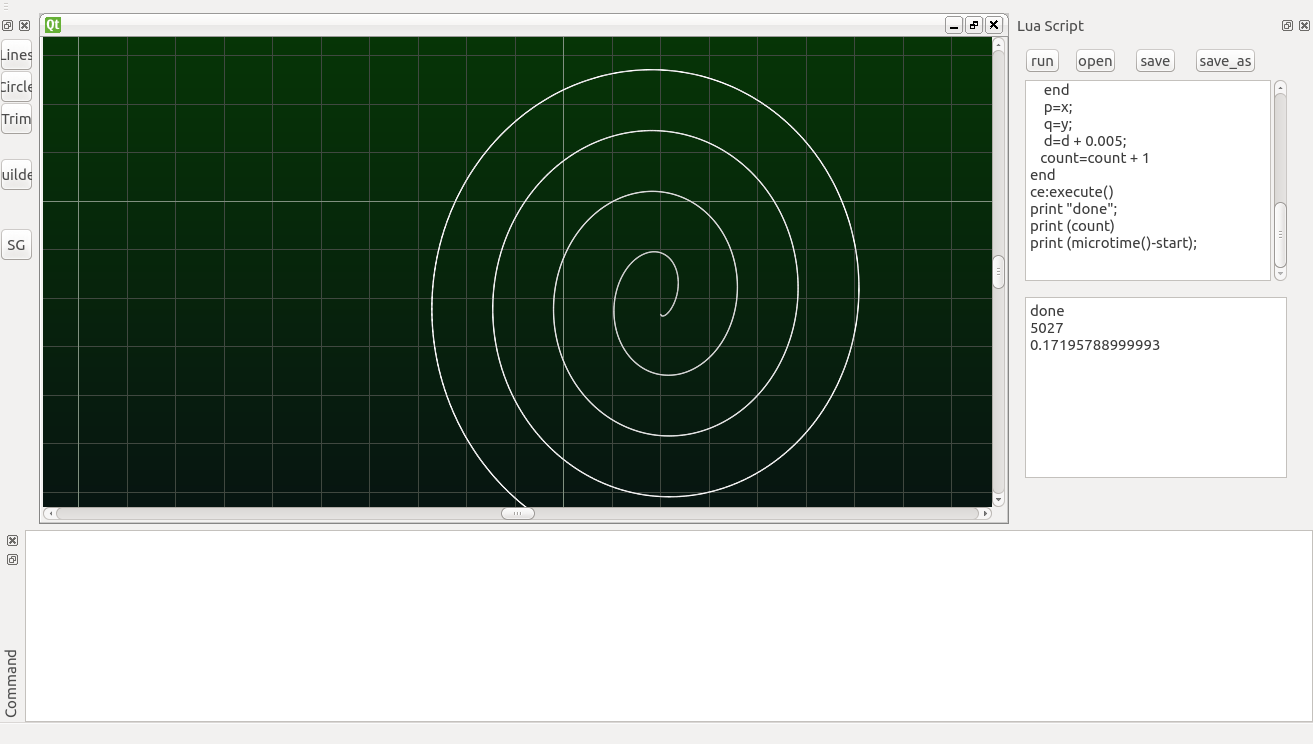
\includegraphics[scale=0.4]{images/ui.png}
\caption{LibreCAD v3 Load/Save Feature}
\end{figure}

\subsubsection{Open}
In this, I added Open feature to LibreCAD v3. This adds a button to the User Interface. When it is clicked, it prompts for a file to be opened. Then choose existing file and click "open". The file will be opened in Lua Script input window so that when the user can click on the run button the script will be run.\\
\begin{figure}[!ht]
\centering
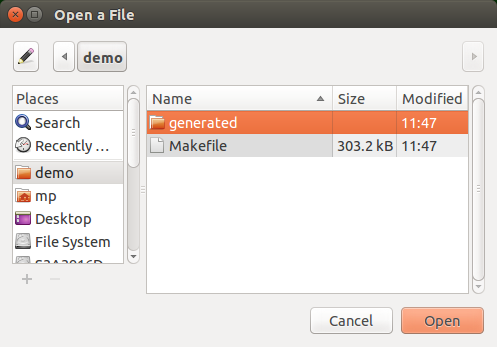
\includegraphics[scale=0.5]{images/open.png}
\caption{Open a File Prompt Box}
\end{figure}

\subsubsection{Save As}
In this feature, when user clicks on "Save As" button, it prompts for a file location on which the file is to be saved and the contents in the Lua Script window are saved in form of a file.
\begin{figure}[!ht]
\centering
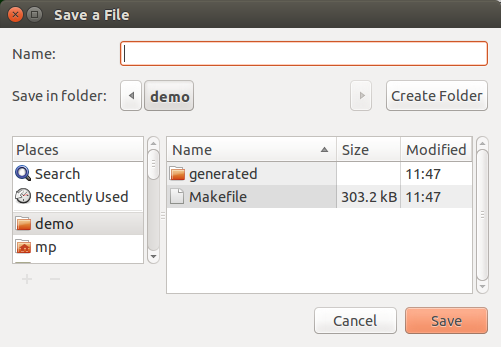
\includegraphics[scale=0.5]{images/save.png}
\caption{Save As Prompt Box}
\end{figure}

\subsubsection{Save}
In this feature, when user clicks on save button, it saves the changes made to the existing file.
